%----------------------------------------------------------------------------------------
%    TITLE PAGE
%----------------------------------------------------------------------------------------

\title{Persistência de Dados}

\author{Prof. Gabriel Rodrigues Caldas de Aquino}

\institute
{
    gabrielaquino@ic.ufrj.br\\
    
    Instituto de Computação -
    Universidade Federal do Rio de Janeiro % Your institution for the title page
}
\date{Compilado em: \\ \today} % Date, can be changed to a custom date

%----------------------------------------------------------------------------------------
%    PRESENTATION SLIDES
%----------------------------------------------------------------------------------------

%------------------------------------------------
\section{Persistência de Dados}
%------------------------------------------------

\begin{frame}
    % Print the title page as the first slide
    \titlepage
\end{frame}



\begin{frame}{Persistência de Dados}
    \begin{block}{Problema}
        Os dados gerados em uma execução do código são perdidos quando o programa é encerrado.
    \end{block}
    
    \begin{block}{Solução}
        Se precisamos usar os dados no futuro, é necessário armazená-los de forma persistente.
    \end{block}
    
    \vspace{0.5cm}
    
    \textbf{Mecanismos de Persistência de Dados:}
    \begin{itemize}
        \item Arquivos (TXT, CSV, JSON, XML)
        \item Bancos de dados (SQLite, PostgreSQL, MySQL)
    \end{itemize}
\end{frame}

\begin{frame}{Persistência em Arquivos de Texto}
    \begin{block}{Características}
        \begin{itemize}
            \item Formatos comuns: \texttt{.txt}, \texttt{.csv}, \texttt{.json}
            \item Armazenamento disco rígido
            \item Manipulação via objetos da classe \texttt{File}
        \end{itemize}
    \end{block}
    
    \begin{exampleblock}{Para manipular temos um "protocolo" de Uso}
        Três etapas: \textbf{Abrir}, \textbf{Manipular} e \textbf{Fechar}

    \end{exampleblock}
    
\end{frame}

\begin{frame}{Fluxo para se fazer a manipulação de arquivos}
    \centering
    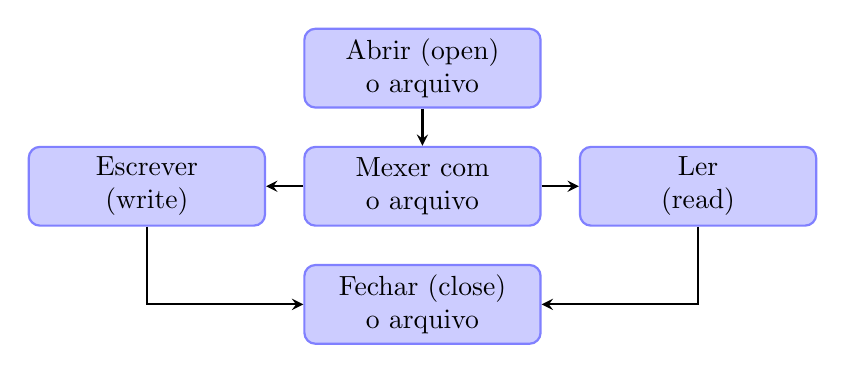
\begin{tikzpicture}[
        node distance=1.5cm,
        etapa/.style={
            rectangle,
            rounded corners,
            draw=blue!50,
            fill=blue!20,
            thick,
            minimum width=3cm,
            minimum height=1cm,
            align=center
        },
        arrow/.style={->, >=stealth, thick}
    ]
    
    \node[etapa] (abrir) {Abrir (open) \\ o arquivo};
    \node[etapa, below of=abrir] (mexer) {Mexer com \\ o arquivo};
    \node[etapa, left of=mexer, xshift=-2cm] (escrever) {Escrever \\ (write)};
    \node[etapa, right of=mexer, xshift=2cm] (ler) {Ler \\ (read)};
    \node[etapa, below of=mexer] (fechar) {Fechar (close) \\ o arquivo};
    
    \draw[arrow] (abrir) -- (mexer);
    \draw[arrow] (mexer) -- (escrever);
    \draw[arrow] (mexer) -- (ler);
    \draw[arrow] (escrever) |- (fechar);
    \draw[arrow] (ler) |- (fechar);
    
    \end{tikzpicture}

    
   
\end{frame}


\begin{frame}[fragile]{Abrindo Arquivos em Python}
    \begin{block}{Método \texttt{open()}}
        Usado para abrir um arquivo. Requer dois parâmetros principais:
\begin{verbatim}
    arquivo = open("nome_do_arquivo.txt", "modo_de_abertura")
\end{verbatim}
        
    \end{block}
    
    \begin{columns}[T]
        \begin{column}{0.5\textwidth}
            \begin{exampleblock}{Parâmetros}
                \begin{itemize}
                    \item \textbf{Nome do arquivo}: \begin{itemize}
                        \item Caminho completo ou relativo
                    \end{itemize}
                    \item \textbf{Modo de abertura}:
                    \begin{itemize}
                        \item \texttt{"r"} - Leitura 
                        \item \texttt{"w"} - Escrita 
                    \end{itemize}
                \end{itemize}
            \end{exampleblock}
        \end{column}
        
        \begin{column}{0.5\textwidth}
            \begin{alertblock}{Exemplos}
\begin{verbatim}
   
# Para escrita
arq = open("dados.txt", "w")

# Para leitura
arq = open("dados.txt", "r")

\end{verbatim}
            \end{alertblock}
        \end{column}
    \end{columns}
    
    \vspace{0.3cm}
    

\end{frame}
\begin{frame}{Modos de Abertura de Arquivos}
    \begin{block}{}
        O modo de abertura define como interagiremos com o arquivo:
    \end{block}

    \centering
    \begin{tabular}{|l|l|l|}
        \hline
        \textbf{Modo} & \textbf{Descrição} & \textbf{Existência do Arquivo} \\
        \hline
        \texttt{r} & Leitura apenas & Deve existir \\
        \hline
        \texttt{w} & Escrita & Cria se não existir \\
        \hline
        \texttt{a} & Escrita no final & Cria se não existir \\
        \hline
        \texttt{r+} & Leitura e escrita & Deve existir \\
        \hline
        \texttt{w+} & Leitura e escrita  & Cria se não existir \\
        \hline
        \texttt{a+} & Leitura e escrita no final & Cria se não existir \\
        \hline
    \end{tabular}
    
\end{frame}


\begin{frame}{Modos de Abertura de Arquivo}

\centering
\includegraphics[width=0.8\textwidth]{Images/diagrama-modos-leitura.png}


\end{frame}


\begin{frame}[fragile]{Abrindo Arquivos - Modo de abertura 'r'}
\begin{itemize}
    \item Método read: ler dados de um arquivo que foi previamente aberto para leitura
    \item Para abrir um arquivo para leitura: 
    \begin{itemize}
        \item Precisamos dar o nome de um arquivo existente 
        \item Em seguida indicar o modo de leitura \textit{r} no momento da abertura
    \end{itemize}

\end{itemize}

\begin{block}{Abrindo o arquivo dados.txt}
\begin{verbatim}
arquivo = open("dados.txt", "r")
conteudo = arquivo.read()
print(conteudo)
arquivo.close()
\end{verbatim}
\end{block}

\end{frame}



\begin{frame}[fragile]{Lendo linha por linha}

\begin{itemize}
    \item Em arquivos com múltiplas linhas podemos usar for loop para facilitar o tratamento linha por linha
\end{itemize}
    
\begin{exampleblock}{Exemplo de leitura linha por linha}
\begin{verbatim}
arquivo="dados.txt"
arq = open(arquivo, "r")
numero_da_linha = 1
for linha in arq:
    print(f"Linha {numero_da_linha}: {linha}")
    numero_da_linha = numero_da_linha + 1
arq.close()
\end{verbatim}
\end{exampleblock}


\end{frame}

\begin{frame}[fragile]{Escrever em Arquivo: write() - Modo de abertura 'w'}

\begin{block}{Método write()}
\begin{verbatim}
arq.write("conteúdo que será escrito no arquivo")
\end{verbatim}
\end{block}

\begin{block}{Passos para escrita em arquivo}
\begin{enumerate}
\item Abrir o arquivo em modo de escrita (\texttt{'w'})
\item Passar o conteúdo como string para \texttt{write()}
\item Fechar o arquivo
\end{enumerate}
\end{block}

\end{frame}

\begin{frame}[fragile]{Escrita Básica em Arquivos}
\begin{block}{Exemplo de escrita em arquivo}
\begin{verbatim}
arq = open("nomes.txt", "w")
arq.write("Gabriel, Pedro, Manoel")
arq.close()
\end{verbatim}
\end{block}

\begin{block}{Importante!}
\begin{itemize}
\item \texttt{'w'} = write (escrita)
\item Sempre feche o arquivo após escrever
\item Cada \texttt{write()} grava o conteúdo exato
\item Se o arquivo "nomes.txt" \textbf{já existe}, ele será \textbf{sobrescrito}
\end{itemize}
\end{block}
\end{frame}

\begin{frame}[fragile]{Arquivos com mais de uma linha}

\begin{block}{Leitura de Arquivos Linha por Linha}
\begin{itemize}
    \item Arquivos com múltiplas linhas contêm \texttt{\textbackslash n} escondido

\end{itemize}
\end{block}

\begin{exampleblock}{Exemplo Prático}
Pedro\textbackslash n

Antonio\textbackslash n

Maria\textbackslash n

Jose\textbackslash n
\end{exampleblock}

\end{frame}

\begin{frame}[fragile]{Pulando linha na escrita em arquivos}

\begin{block}{Código de exemplo}
\begin{verbatim}
arq = open("nomes.txt", "w")
arq.write("Gabriel\nPedro\nManoel")
arq.close()
\end{verbatim}
\end{block}



\begin{alertblock}{O que acontece?}
\begin{itemize}
\item \texttt{\textbackslash n} é o \textbf{caractere especial} para quebra de linha
\item Quando escrito no arquivo, ele:
  \begin{itemize}
  \item Finaliza a linha atual
  \item Move o cursor para a próxima linha
  \end{itemize}

\end{itemize}
\end{alertblock}


\end{frame}

\begin{frame}[fragile]{Fechando o Arquivo: close()}

\begin{block}{Método close()}
\begin{verbatim}
arq.close()  # Fecha o arquivo após uso
\end{verbatim}
\end{block}

\begin{alertblock}{Por que fechar arquivos?}
\begin{itemize}
\item \textbf{Libera recursos do sistema}: Arquivos abertos consomem memória
\item \textbf{Garante a escrita completa}: Dados podem ficar em buffer
\item \textbf{Evita corrupção}: Previne acesso concorrente indevido
\item \textbf{Libera o arquivo}: Permite que outros programas o acessem
\end{itemize}
\end{alertblock}


\end{frame}


\begin{frame}[fragile]{Modo de Abertura 'a' (Append)}
    \begin{block}{Funcionamento do modo \texttt{"a"}}
        \begin{verbatim}
arquivo = open("dados.txt", "a")  # Modo append
arquivo.write("Novo conteúdo\n")
arquivo.close()
        \end{verbatim}
    \end{block}

            \begin{alertblock}{Características}
                \begin{itemize}
                    \item \textbf{Abre para escrita} no final do arquivo
                    
                    \item Ponteiro no \textbf{fim do arquivo} (só escreve no final)
                \end{itemize}
            \end{alertblock}

        

\end{frame}


\begin{frame}[fragile]{Gerenciamento de Arquivos com \texttt{with open}}
    \begin{block}{Sintaxe Básica}
        \begin{verbatim}
with open("arquivo.txt", "modo") as arquivo:
    # Bloco de código
        \end{verbatim}
    \end{block}

            \begin{exampleblock}{Exemplo Prático}
                \begin{verbatim}
with open("dados.txt", "r") as arq:
    conteudo = arq.read()
    print(conteudo)
                \end{verbatim}
            \end{exampleblock}
   

    \begin{block}{Facilidade}
    \begin{itemize}
        \item O \texttt{with} deixa arquivo aberto.
        \item Ao sair do bloco, o \texttt{close()} é  automático.
    \end{itemize}
         
    \end{block}
\end{frame}

\begin{frame}[fragile]{Controlando a Posição com \texttt{seek()}}

    \begin{block}{O que é \texttt{seek()}?}
        Método que permite mover o "cursor" de leitura/escrita para qualquer posição no arquivo
        \begin{verbatim}
arquivo.seek(offset)
        \end{verbatim}
    \end{block}

  
            \begin{alertblock}{Parâmetros}
                \begin{itemize}
                    \item \textbf{offset}: Número de bytes para mover
                    
                \end{itemize}
            \end{alertblock}
      
            \begin{exampleblock}{Exemplos}
                \begin{verbatim}
# Ir para o byte 10
arquivo.seek(10)
                \end{verbatim}
            \end{exampleblock}
 


    
   
\end{frame}

\begin{frame}[fragile]{Modo de Abertura \texttt{r+}}

\begin{block}{Funcionamento do modo \texttt{"r+"}}
\begin{verbatim}
with open("arquivo.txt", "r+") as arquivo:
    # Operações de leitura E escrita
    conteudo = arquivo.read()  # Lê
    arquivo.write("novo texto")  # Escreve
\end{verbatim}
\end{block}

        \begin{alertblock}{Características}
            \begin{itemize}
                \item Permite \textbf{leitura e escrita} no mesmo arquivo
               \item Não apaga o arquivo na hora de abrir
                \item Posição inicial: \textbf{início do arquivo}
            \end{itemize}
        \end{alertblock}

\end{frame}

\begin{frame}[fragile]{Modo de Abertura \texttt{w+} (Escrita e Leitura)}
    \begin{block}{Funcionamento do modo \texttt{"w+"}}
        \begin{verbatim}
with open("arquivo.txt", "w+") as arquivo:
    arquivo.write("Conteúdo inicial\n")
    arquivo.seek(0)  # Volta ao início para leitura
    conteudo = arquivo.read()
    print(conteudo)
        \end{verbatim}
    \end{block}

    \begin{columns}[T]
        \begin{column}{0.5\textwidth}
            \begin{alertblock}{Características Principais}
                \begin{itemize}
                    \item \textbf{Apaga conteúdo existente}
                   
                    \item Posição inicial: \textbf{início do arquivo}
                    
                \end{itemize}
            \end{alertblock}
        \end{column}
        
        \begin{column}{0.5\textwidth}
            
            
            \begin{block}{Cuidado!}
                Sempre use \texttt{seek()} antes de ler após escrever
            \end{block}
        \end{column}
    \end{columns}


\end{frame}
\begin{frame}[fragile]{Modo de Abertura \texttt{a+} (Append e Leitura)}

\begin{block}{Funcionamento do modo \texttt{"a+"}}
\begin{verbatim}
with open("arquivo-teste.txt", "a+") as arquivo:
    arquivo.write("Nova entrada\n")  # Escreve no FINAL
    arquivo.seek(0)                  # Volta ao início
    texto = arquivo.read()       # Lê todo conteúdo
    print(texto)
\end{verbatim}
\end{block}

        \begin{alertblock}{Características}
            \begin{itemize}
               \item \textbf{Não apaga} conteúdo existente 
               \item Posição inicial:  \textbf{Final do arquivo}
                
            \end{itemize}
        \end{alertblock}
\end{frame}




\begin{frame}[fragile]{Tratamento de Exceções com Arquivos}

\begin{block}{Por que tratar exceções?}
Lidar com arquivos pode lançar exceções inesperadas que devem ser gerenciadas.
\end{block}

\begin{block}{Principais exceções com arquivos}
\begin{itemize}
\item \texttt{FileNotFoundError}: Arquivo não existe ou caminho incorreto
\item \texttt{IOError}: Erros gerais de entrada/saída (disco cheio, permissões)
\end{itemize}
\end{block}




\end{frame}

\begin{frame}[fragile]{Tratamento de Exceções com Arquivos}

\begin{block}{Código de Exemplo}
\begin{verbatim}
try:
    f = open("arquivo-inexistente.txt", "r")
    conteudo = f.read()
    f.close()
    print(conteudo)
except FileNotFoundError:
    print("Arquivo não existente")
\end{verbatim}
\end{block}




\end{frame}

\begin{frame}[fragile]{Demonstração: Tratando Arquivo Corrompido}

\begin{block}{Código de Tratamento}
\begin{verbatim}
try:
    f = open("arquivo-corrompido.txt", "r")
    conteudo = f.read()
    f.close()
    print(conteudo)
except IOError:
    print("Erro: Problema ao ler o arquivo")
\end{verbatim}
\end{block}


\end{frame}

